\chapter{ \MakeUppercase{Clasificación supervisada de ruido en muografía por pérdida de energía.}}
\label{ch:e_rapido}

En esta sección se muestra la clasificación de los eventos detectados por MuTe mediante algoritmos de aprendizaje supervisado. En este apartado se hace un recuento de los métodos y propuestas que se emplearon para concluir la primera etapa, con los resultados y los problemas que surgieron durante su desarrollo.

\section{Extracción de características.}

La extracción de características se basa en la parametrización y análisis de los datos suministrados por el WCD por medio de un histograma de carga. A continuación se presentan los pasos empleados:

\alglanguage{pseudocode}
\begin{algorithm}[h]
\small
\caption{Extracción de características}
\label{Begin_Read}
\begin{algorithmic}[1]
\State Extraer los datos crudos del detector y posteriormente ordenarlos.
\State Parametrizar los datos para ajustarlo a una distribución probabilística.
\State Implementar un histograma de carga, para identificar y separar la componente muónica de la electromagnética y multipartícula.
\State Encontrar características según los resultados de las variables de entrada de cada componente.
\Statex
\end{algorithmic}
  \vspace{-0.1cm}
\end{algorithm}

 
\section{Discriminación entre muones, componente electromagnética\\ y multi-partícula.}

Las características (la carga de las componentes, la variaza y la media) se ajustan a diferentes modelos de clasificación como: \textit{naive gaussian}, \textit{suport vector machine}, \textit{random forest} y \textit{gaussian mixture model}. Se etiquetan como componente: muónica, electromagnética y multi-partícula. Para ello se emplearon los siguientes pasos:

\alglanguage{pseudocode}
\begin{algorithm}[h]
\small
\caption{Discriminación entre muones, electromagnética y multi-partícula.}
\label{Begin_Read}
\begin{algorithmic}[1]
\State Definir una función de probabilidad optimizando los valores que ajusten a la curva de la distribución seleccionada.
\State A partir de los valores ajustados con la función de densidad de probabilidad (PDF), analizar independientemente cada componente por medio de la distribución extraída del histograma de carga.
\State Se etiqueta cada tupla de datos que se  representan como: 1 para mounes, 0 para electromagnético y 2 para multi-partícula.
\State Para el entrenamiento de los datos se emplean los siguientes modelos de clasificación: \textit{naive gaussian}, \textit{suport vector machine}, \textit{random forest} y \textit{gaussian mixture model}. Donde se utilizan las características (la carga de las componentes, la variaza y la media) y etiquetas, de tal manera que se pueda evaluar el comportamiento del clasificador a usar\footcite{perez2005modelos}.
\Statex
\end{algorithmic}
  \vspace{-0.1cm}%
\end{algorithm}


\section{Minería de datos}
Inicialmente la base del problema se encuentra en el reconocimiento de los datos entregados por el WCD. Los datos están dados por los valores de carga (energía depositada). Los datos se modelaron con histogramas de frecuencia de carga, de dos dimensiones (Carga vs Frecuencia), como se muestra en la Fig. \ref{uno}. El histograma evidencia tres componentes, que guiados por un conocimiento a priori, se clasifican como (muónica, electromagnética y multi-partícula).\\

%Se cargan los datos crudos implementando histogramas donde se proyecta la cantidad de datos.
%-El modelo fue creado a partir de los datos de carga con el histograma de Frecuencia de la Carga (eje X), simulando los datos crudos (llamados \textit{Carga1}), ya que, al inicio del proyecto no se contaba estos. Cabe resaltar que se hizo la prueba del modelo, se obtuvieron resultados y de estos resultados, conclusiones. Todo esto a partir de los datos crudos de Carga.-\\ 

\begin{figure}[h!]
\begin{center}
\caption {Histograma de carga para un registro de datos de una hora del WCD de MuTe. (arriba).  Datos del WCD de eventos que han atravesado el hodoscopio (abajo).}
\includegraphics[width=0.7
\textwidth]{Figures/imagenes/1.png}
\label{uno}
\end{center}
\end{figure}

Al recibir los datos crudos totales, se hizo el procesamiento y modelamiento de los datos para implementarlos en el modelo GMM ya ajustado con los datos de carga del histograma. El modelo presentó complicaciones para evidenciar las componentes, esto se presentó debido a un grupo de datos innecesarios (outliers). Separando y visualizando los datos crudos, se estableció un límite donde sólo se tuvo en cuenta valores de carga $<$ 800 ADC.bin, ya que por encima de esto los datos no aportaban información relevante (ver Fig. \ref{dos}).

\begin{figure}[h]
\begin{center}
\caption{Datos de Carga crudos. ARRIBA: Datos completos de carga.  ABAJO:.Datos acotados por el umbral (Carga $<$ 800)}
\includegraphics[width=0.6\textwidth]{Figures/imagenes/2.png}
\label{dos}
\end{center}
\end{figure}


\section{Modelo de mezcla de gaussianas y parametrización}

Los modelos de mezcla gaussiana (GMM), representan subpoblaciones normalmente distribuidas dentro de una población general. Este modelo parametriza un subconjunto que pertenece a un grupo de datos. GMM puede tener más de 2 componentes y estima los parámetros individuales para modelar por medio de distribuciones normales.

GMM necesita parámetros iniciales para obtener un mejor ajuste. Los parámetros más usados en este caso fueron: el número de componentes, el peso de cada una de las componentes, el número de inicializaciones que debe hacer y el número de iteraciones. Cuando el GMM converge retorna valores como las medias, varianzas y el peso de cada una de las componentes. Adicionalmente, se ajustó una PDF a cada componente, (muónica, electromagnética y multi-partícula) permitiendo comparar los resultados con los datos. 

En la primera separación de las componentes se evidenció que el modelo con pocos datos (1.323) no responde acertadamente. Pero al contar con la cantidad total de los datos (1'273.125), el modelo mostró un mejor ajuste. 

\begin{figure}[h!]
\begin{center}
\caption{Histograma de frecuencia con los datos y la función de densidad de probabilidad ajustada por GMM. Con las medias calculadas, para apreciar el ajuste a los datos.}
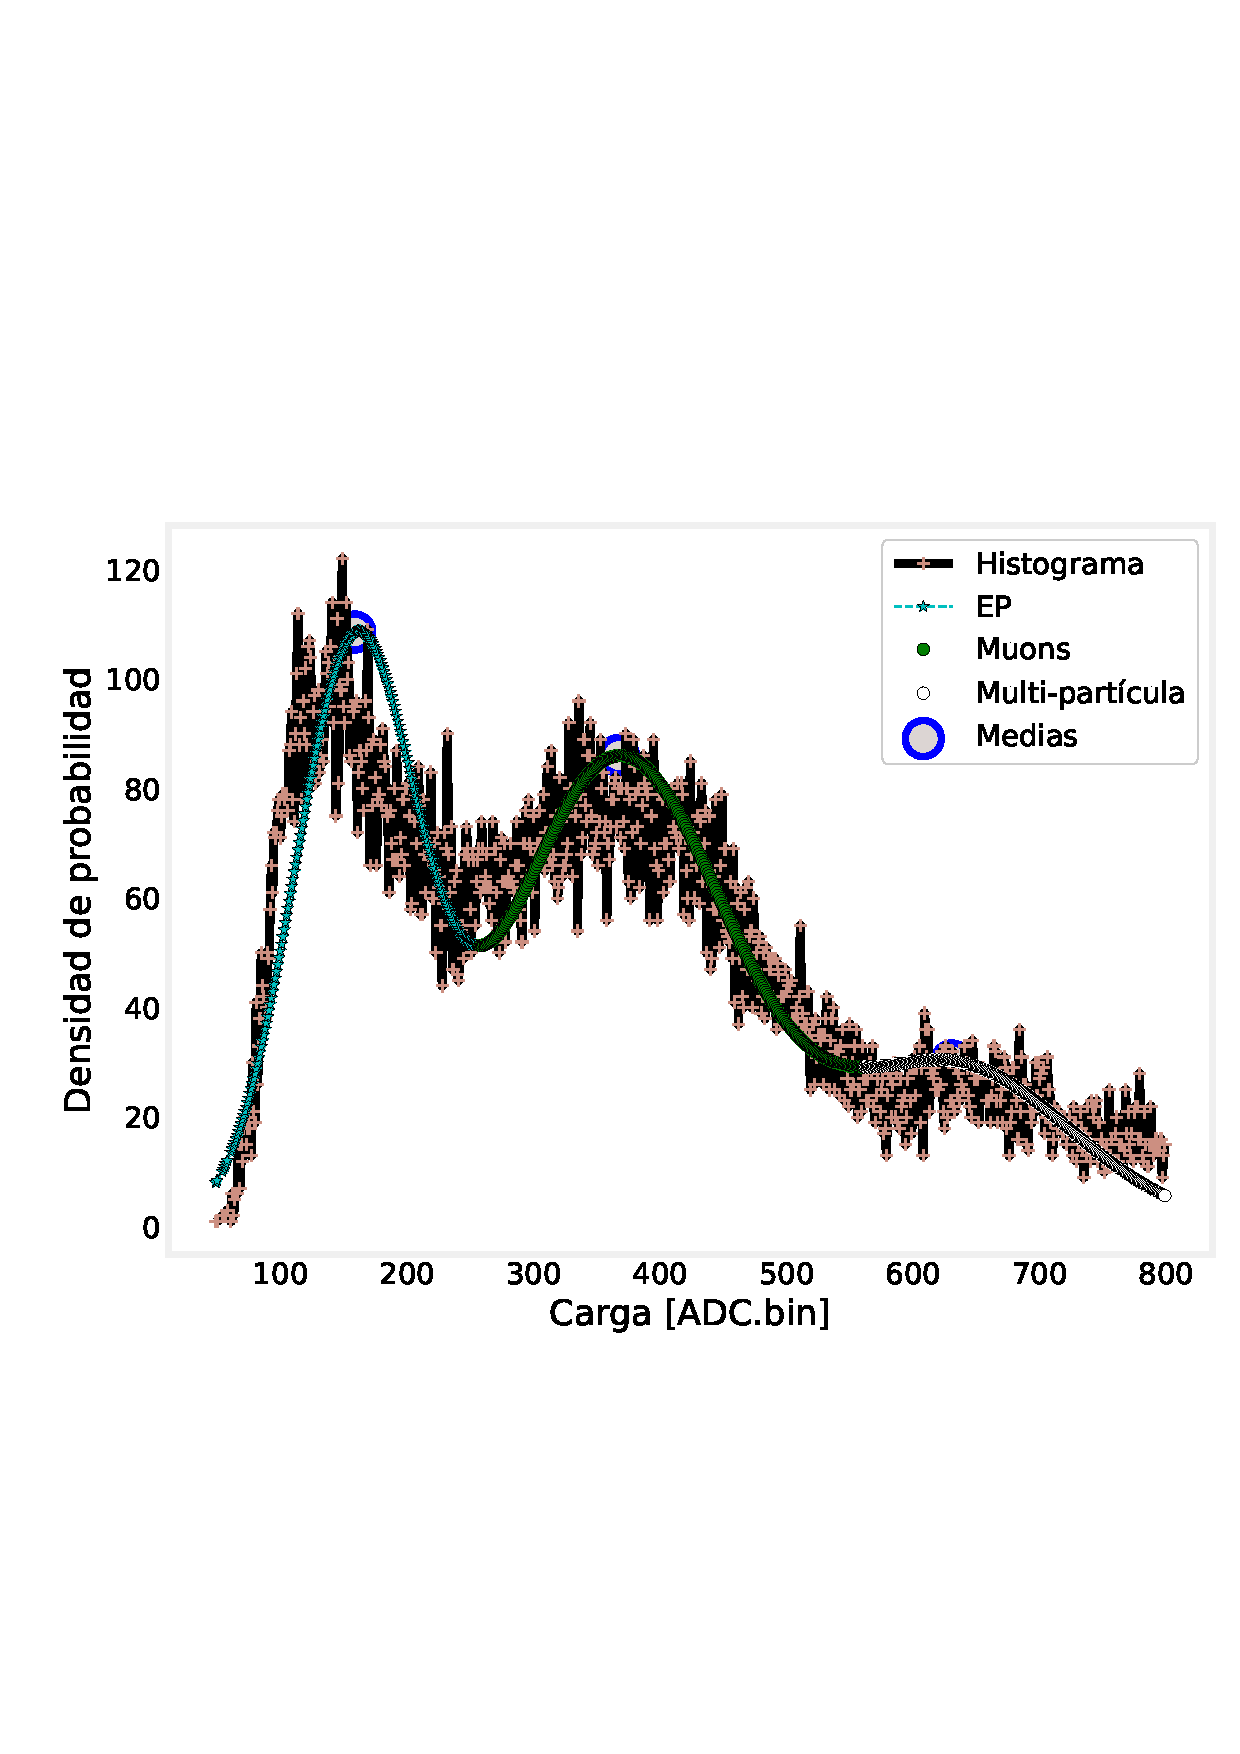
\includegraphics[width=0.7\textwidth]{Figures/imagenes/4.png}
\label{cuatro}
\end{center}
\end{figure}

%Los primeros datos procesados fueron \textit{Carga1}, que cumplían la función de entregar valores de carga, pero no había valores repetidos, puesto que se extraían del histograma de frecuencia limitando y confundiendo a GMM. Todo el modelo se construyó con los datos de \textit{Carga1} (al principio del proyecto)ver Fig.\ref{tres}, se hizo para tener una base al momento de agrupar todos los datos reales, para ajustar el modelo al ingresar los datos de \textit{Carga2}. ver Fig. \ref{cuatro}.%

%Con los resultados obtenidos de GMM se pudo avanzar de una formas más fácil y precisa, ya que se parametrizaron cada una de las gaussianas para un manejo independiente mejorando el análisis a lo largo del proyecto. %


\section{Construcción de gaussianas y etiquetado}

Con los parámetros de cada una de las gaussianas obtenidos previamente, se creó una función gaussiana definida por la Ecuación (\ref{P.D.F}) de densidad de probabilidad.
\begin{equation}
f(x)=A*e^{-\frac{1}{2}(\frac{x-\mu}{\sigma})^2}
\label{P.D.F}
\end{equation}
donde A es la escala, $\mu$ la media, $\sigma$ la varianza y x los datos. Se definieron tres funciones para las tres componentes (EP, muón y multi-partícula) como se muestra en la Fig. \ref{cinco}


Definidas las tres funciones se analizan independientemente etiquetando: 0 para muon, 1 para electromagnético y 2 para multi-partícula. Se crea un vector con las etiquetas de la misma longitud del vector carga.

\begin{figure}[h!]
\centering
\begin{center}
\caption{ Las tres componentes: la muónica (verde),  la electromagnética (azul) y multi-partícula (roja), representadas por su respectiva función de densidad de probabilidad.}
\includegraphics[width=0.7\textwidth]{Figures/imagenes/5.png}
\label{cinco}
\end{center}
\end{figure}
\section{Clasificación supervisada, división y entrenamiento}\\

Con los datos etiquetados se debe hacer un \textit{Split} para entrenar el clasificador. En este proyecto se usó \textit{Train Test Split} implementado en la librería de \textit{SKlearn}, ya que además de cumplir con el objetivo principal es una herramienta fácil y rápida de usar. Los datos fueron separados en dos conjuntos, Test (70\% de datos) y train (30\% de datos) para evaluar los modelos de clasificación. \\

En este caso se usaron tres modelos de clasificación supervisada: \textit{Naive Gaussian, RandomForest y Support Vector Machines} implementados en la librería \textit{SKlearn}. Los clasificadores se evaluaron mediante métricas de la matriz de confusión y eficiencia. Se generaron visualizaciones gráficas. (ver Fig. \ref{seis}).\\
\\

\begin{figure}[h]
\begin{center}
\caption{Resultados del etiquetado de los datos por el clasificados y ajuste de las distribuciones.}
\includegraphics[width=0.8\textwidth]{Figures/imagenes/6ta.png}

\label{seis}
\end{center}
\end{figure}\\


En la matriz de confusión de la Tabla (\ref{mat}) se muestra el resultado obtenido por el clasificador. Los valores erróneos se dan entre las componentes estrictamente contiguas, como lo es la electromagnético con muónica y la muónica con la multi-partícula. No hubo fallos en la predicción entre muón y multi-partícula. \\

\begin{table}[t]
\begin{center}
\caption{Matriz de confusión del \textit{naive gaussian}. Donde las columnas 1, 2 y 3 son valores reales que representan las componentes: electromagnética, muónica y multi-partícula. Las filas 1, 2 y 3 son los valores predichos que definen las componentes electromagnética, muónica y multi-partícula.}
\begin{tabular}{| c | c | c | c | }
\hline
 & Electromagnética & Muón & Multi-partícula\\
 \hline
 Electromagnética & 4026 & 49 & 0\\
\hline
 Muón & 0 & 5297 & 0\\
\hline
Multi-partícula & 0 & 51 & 1702 \\
\hline

\end{tabular}
\label{mat}
\end{center}
\end{table}


El valor de precisión en la Tabla (\ref{pres}) se refiere a cuán cerca del valor real se encuentra el valor medido. En la componente electromagnética y multi-partícula se obtuvo una precisión de 100\%. La muónica se redujo a 98\%: predijo que 49 datos de carga pertenecían a la componente muónica, cuando realmente pertenecían a la componente electromagnética y en 51 casos el clasificador los etiquetó como muónica cuando pertenecía verdaderamente a la componente multi-partícula.

La veracidad o sensibilidad del modelo determina la proporción de los casos positivos clasificados por el modelo con respecto al total de los datos positivos. En esta métrica el clasificador asignó correctamente el 100\% de los datos pertenecientes a la componente muónica. En la componente electromagnética (99\%) obtuvo 4026 verdaderos positivos y 49 falsos positivos (muónica). En la multi-partícula (97\%) se obtuvieron 1702 verdaderos positivos y 51 falsos positivos (muónica).  


\begin{table}[t]
\begin{center}
\caption{Precisión extraídas de la matriz de confusión}
\begin{tabular}{| c | c | c | c | c |}
\hline
 & Precisión & Veracidad & score & Datos \\ \hline
Electromagnético & 1.00 & 0.99 & 0.99 & 4075 \\ \hline
Muón & 0.98 & 1.00 & 0.99 & 5297 \\  \hline
Multi-partícula & 1.00 & 0.97 & 0.99 & 1753 \\\hline

\end{tabular}
\label{pres}
\end{center}
\end{table}





